\documentclass[tikz,border=4pt]{standalone}
\usepackage[T1]{fontenc}
\usepackage{lmodern}
\usetikzlibrary{arrows.meta,calc,positioning}
\ifdefined\darkmode
  \definecolor{paper}{HTML}{17191B}\definecolor{ink}{HTML}{D7D7D3}
  \definecolor{muted}{HTML}{969A9C}\definecolor{accent}{HTML}{7F9EAE}
  \definecolor{solar}{HTML}{C4A56C}\definecolor{line}{HTML}{3B4043}
  \definecolor{panel}{HTML}{202326}
\else
  \definecolor{paper}{HTML}{F5F5F2}\definecolor{ink}{HTML}{202326}
  \definecolor{muted}{HTML}{666B70}\definecolor{accent}{HTML}{315F78}
  \definecolor{solar}{HTML}{8A6428}\definecolor{line}{HTML}{CFD2D2}
  \definecolor{panel}{HTML}{ECEEEC}
\fi
\begin{document}\sffamily
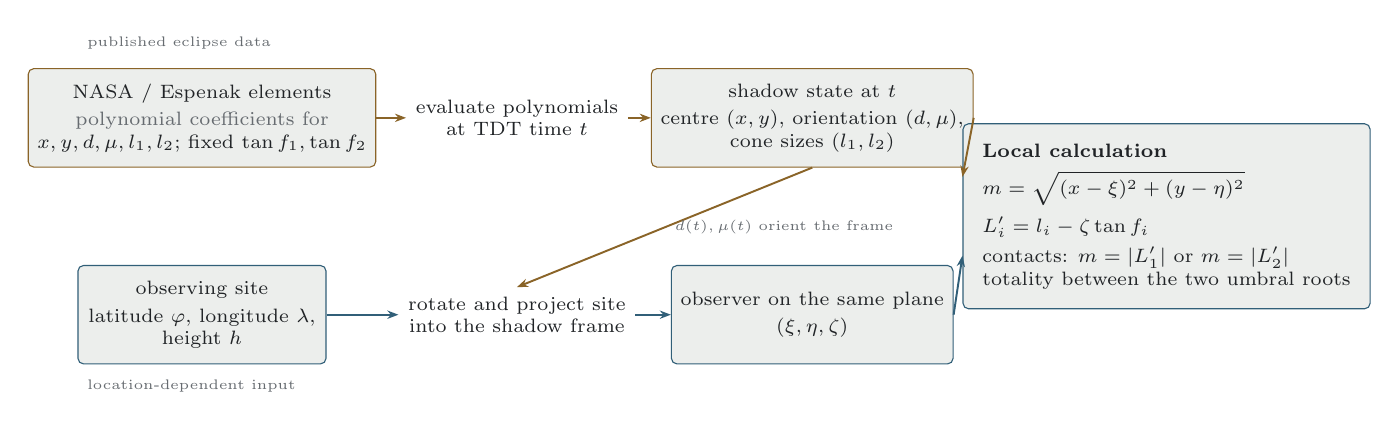
\begin{tikzpicture}[
  data/.style={draw=solar,fill=panel,rounded corners=2pt,text=ink,
    minimum width=3.15cm,minimum height=1.25cm,align=center,font=\scriptsize},
  local/.style={draw=accent,fill=panel,rounded corners=2pt,text=ink,
    minimum width=3.15cm,minimum height=1.25cm,align=center,font=\scriptsize},
  operation/.style={text=ink,align=center,font=\scriptsize},
  result/.style={draw=accent,fill=panel,rounded corners=2pt,text=ink,
    minimum width=4.0cm,minimum height=2.35cm,align=left,font=\scriptsize,inner sep=7pt},
  dataarrow/.style={draw=solar,line width=.7pt,-{Stealth[length=4pt]}},
  localarrow/.style={draw=accent,line width=.7pt,-{Stealth[length=4pt]}},
  note/.style={text=muted,font=\tiny,align=center}
]
\node[data] (nasa) at (0,1.35)
  {NASA / Espenak elements\\[2pt]
   \textcolor{muted}{polynomial coefficients for}\\
   $x,y,d,\mu,l_1,l_2$; fixed $\tan f_1,\tan f_2$};
\node[operation] (eval) at (4.0,1.35)
  {evaluate polynomials\\at TDT time $t$};
\node[data] (shadow) at (7.75,1.35)
  {shadow state at $t$\\[2pt]
   centre $(x,y)$, orientation $(d,\mu)$,\\
   cone sizes $(l_1,l_2)$};

\node[local] (site) at (0,-1.15)
  {observing site\\[2pt]
   latitude $\varphi$, longitude $\lambda$,\\height $h$};
\node[operation] (project) at (4.0,-1.15)
  {rotate and project site\\into the shadow frame};
\node[local] (observer) at (7.75,-1.15)
  {observer on the same plane\\[2pt]
   $(\xi,\eta,\zeta)$};

\node[result] (compare) at (12.25,.10)
  {\textbf{Local calculation}\\[4pt]
   $m=\sqrt{(x-\xi)^2+(y-\eta)^2}$\\[3pt]
   $L'_i=l_i-\zeta\tan f_i$\\[3pt]
   contacts: $m=|L'_1|$ or $m=|L'_2|$\\
   totality between the two umbral roots};

\draw[dataarrow] (nasa)--(eval);
\draw[dataarrow] (eval)--(shadow);
\draw[localarrow] (site)--(project);
\draw[localarrow] (project)--(observer);
\draw[dataarrow] (shadow.east)--([yshift=5mm]compare.west);
\draw[localarrow] (observer.east)--([yshift=-5mm]compare.west);
\draw[dataarrow] (shadow.south) -- node[note,anchor=west] {$d(t),\mu(t)$ orient the frame}
  (project.north);

\node[note,anchor=west] at (-1.58,2.30)
  {published eclipse data};
\node[note,anchor=west] at (-1.58,-2.05)
  {location-dependent input};
\end{tikzpicture}
\end{document}
